\documentclass[11pt,letterpaper]{article}
\usepackage[top=1in,bottom=1in,left=1in,right=1in]{geometry}
\pagestyle{empty}
\usepackage{graphicx}
\usepackage{amsmath}

\usepackage[dvipsnames]{xcolor}
\newcommand{\sol}[1]{{\color{NavyBlue} #1}}
%\newcommand{\sol}[1]{{\color{White} #1}} % uncomment to hide solutions


\begin{document}
\setlength{\parindent}{0cm}
\setlength{\parskip}{11pt}
Exam \#1: Basic kinematics and dynamics

Name: \hfill /30\\

\hrulefill\\
1. In lab you did experiments in which you accelerated a cart down a track by hanging a mass over a pulley, as shown in the figure below. If you hold the cart and start collecting before you let go, you can observe a drop in the force measured by the force probe at the instant that the cart starts accelerating. Why? Consider the forces on the hanging mass to help you answer this question. [6 pts]

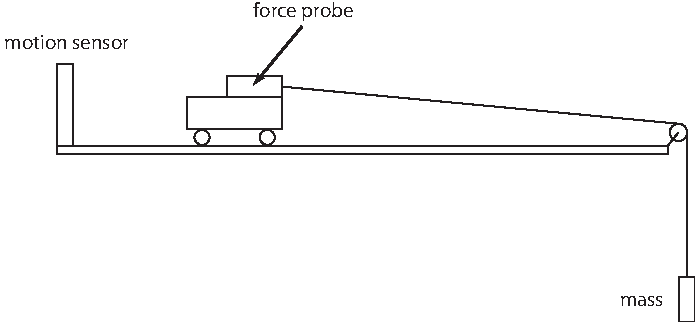
\includegraphics[width=\textwidth]{../../labs/lab3-forces/cart_and_pulley.pdf}

\sol{When the cart is not moving, the sum of the forces on the hanging mass must equal zero.
\begin{equation}
\sum F_y = F_t - F_g = 0 \Rightarrow F_t = mg
\end{equation}
This is no longer true once the cart begins to accelerate, in which case
\begin{equation}
\sum F_y = F_t - F_g = ma_y \Rightarrow F_t = m(g+a_y)
\end{equation}
$a_y$ is negative because the mass is falling in the negative $y$-direction (here assumed to point upward). This means that the tensional force that is resisting the falling motion is reduced by some small amount; if it wasn't, then the mass wouldn't fall.

Because the masses of the string and pulley are small, and the pulleys have very little friction, the tension of the string is the same everywhere, which also means that there must be a reduction in the tensional force pulling on the force probe.

}

\clearpage
2. In the figure below, the particles are traveling counterclockwise in circles of radius 5 m with speeds that may be varying. The acceleration vectors are indicated at certain times. Find the speed and tangential acceleration for both (a) and (b). [6 pts]

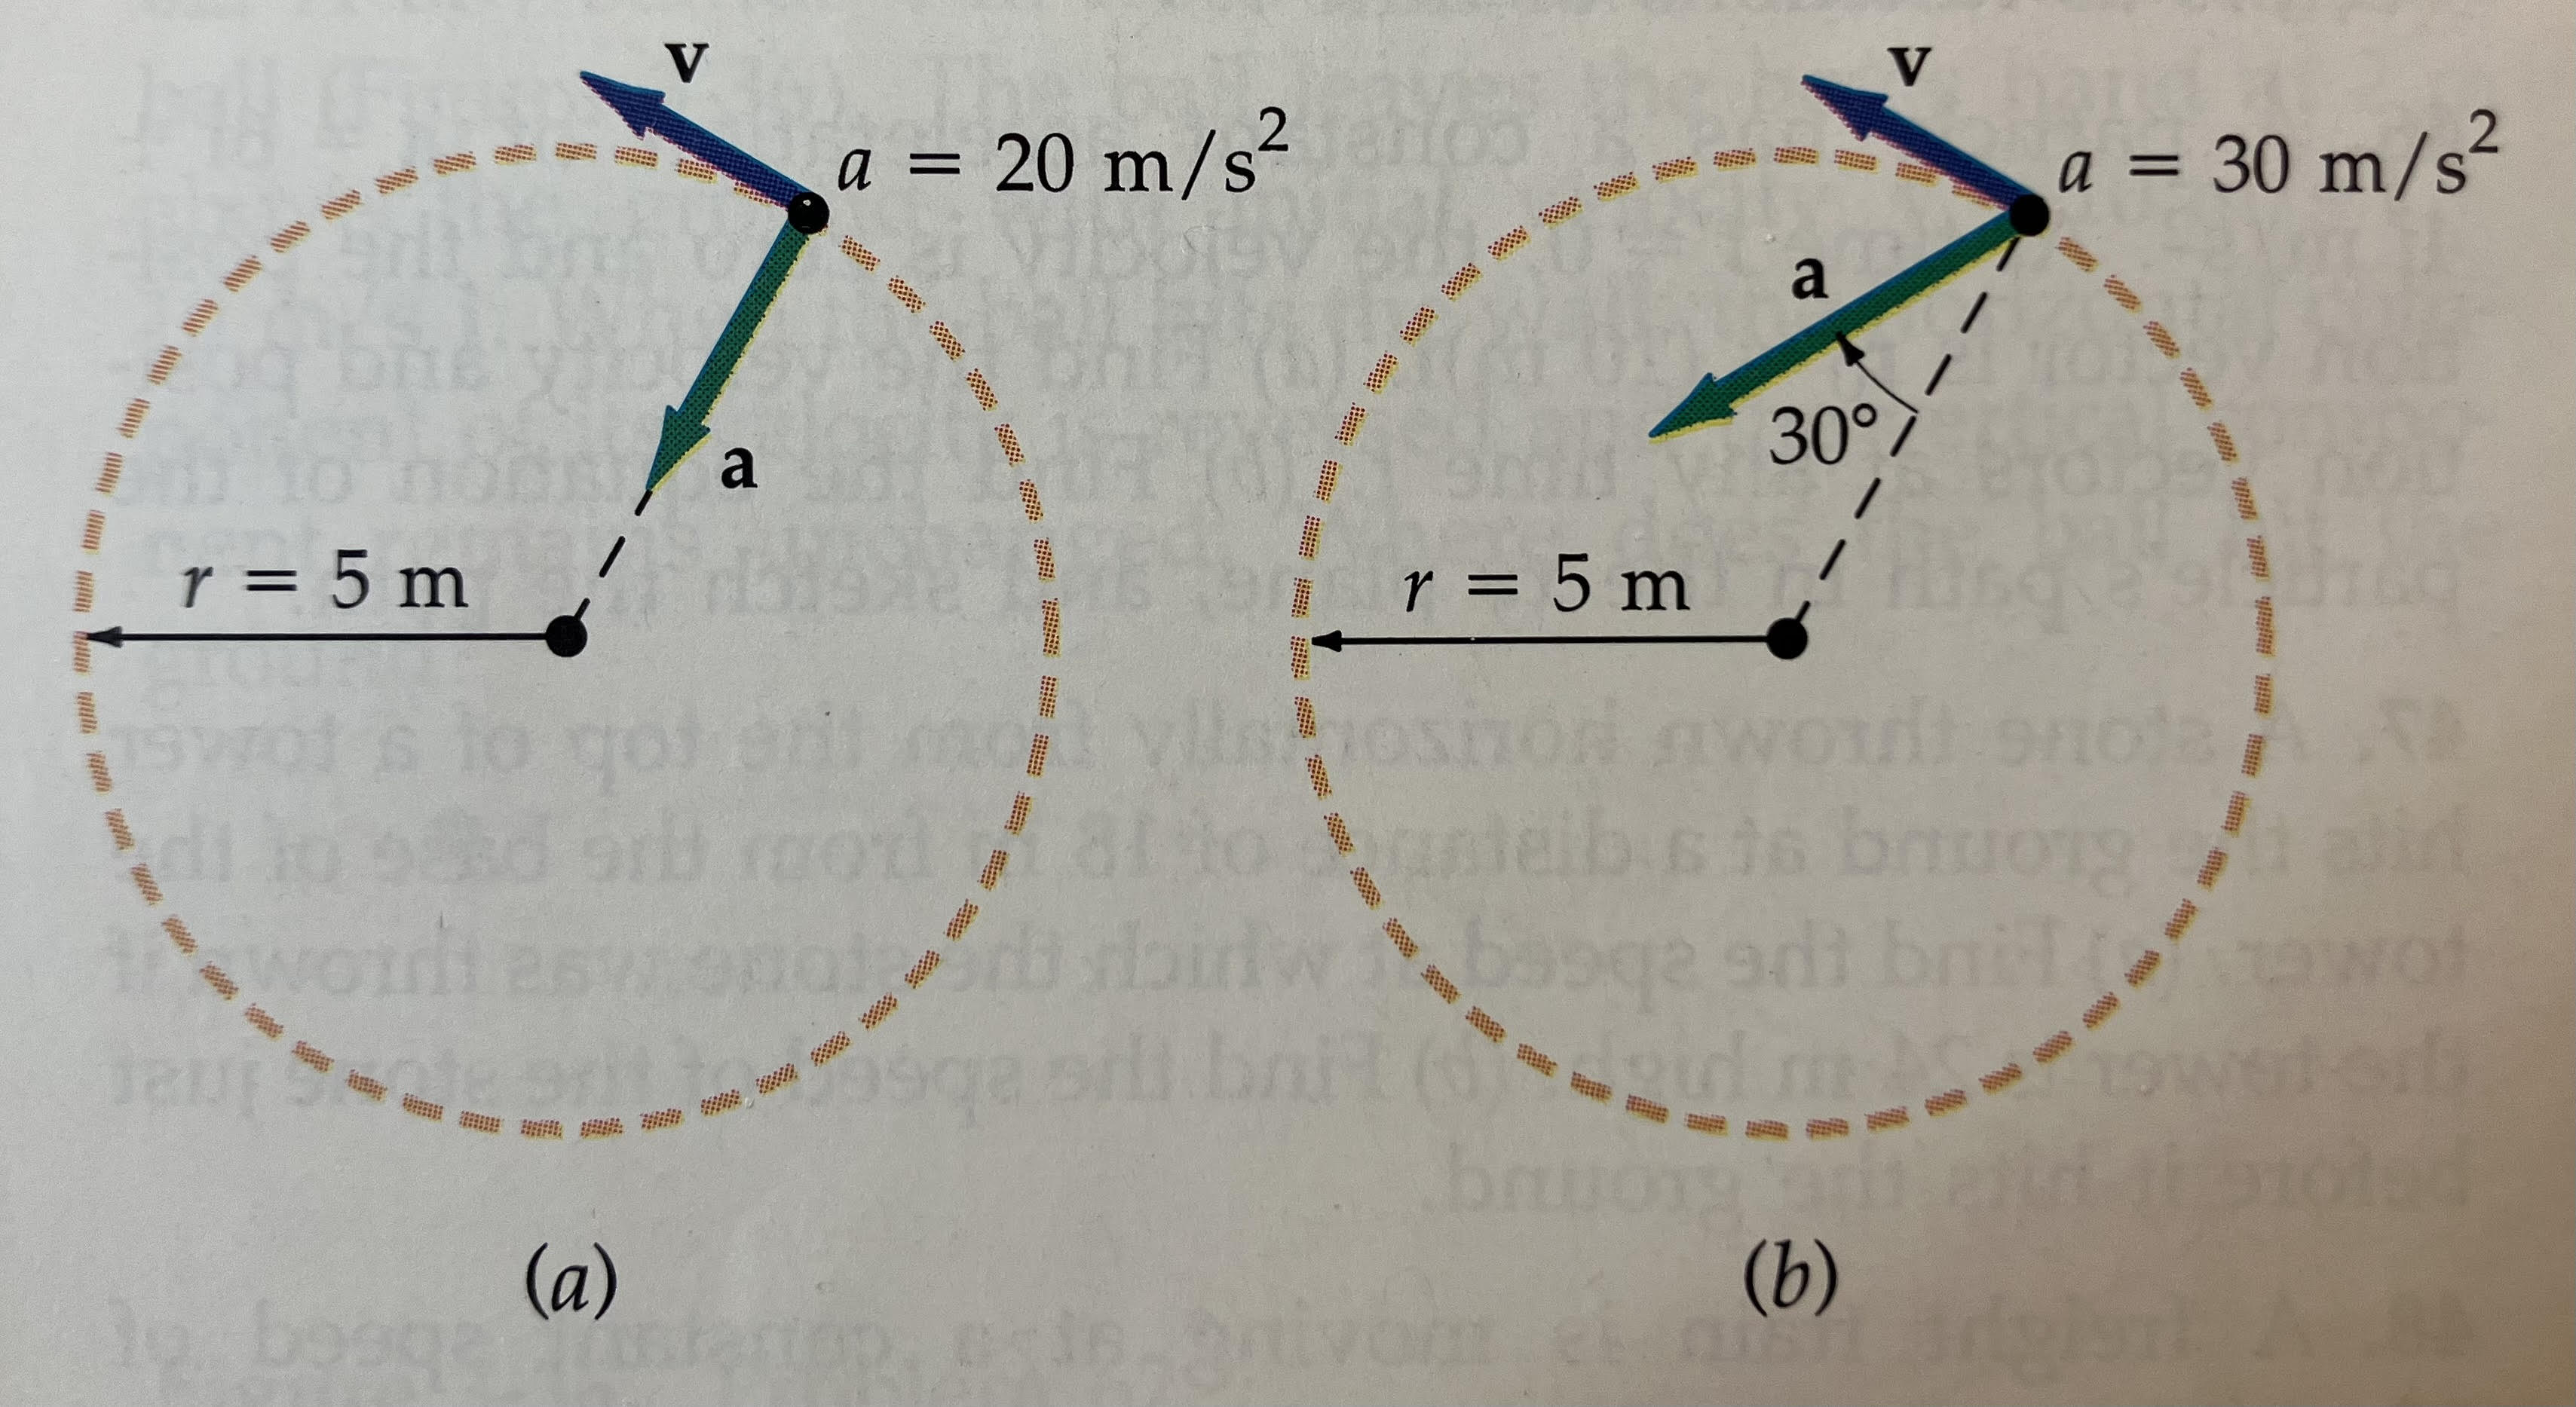
\includegraphics[width=\textwidth]{exam1_2.jpg}

\sol{(a) The acceleration vector is pointing toward the center of the circle, implying that the acceleration the centripetal acceleration and there is no tangential acceleration. This means that
\begin{equation}
\boxed{a_t = 0\mbox{ m/s}^2}
\end{equation}
and 
\begin{equation}
a = a_c = \frac{v^2}{r} \Rightarrow \boxed{v=\sqrt{a_cr}=10\mbox{ m/s}}
\end{equation}

(b) Here, the acceleration vector is not pointing toward the center of the circle, which means that it contains both centripetal and tangential accelerations. The tangential acceleration is the component of the acceleration that points tangential to the circle, which is given by
\begin{equation}
\boxed{a_t = a\sin(30) = 15\mbox{ m/s}^2}.
\end{equation}
The centripetal acceleration is $a_c=a\cos(30) = 26\mbox{ m/s}^2$, and therefore we can calculate the speed $v$ as before:
\begin{equation}
a_c = a\cos(30) = \frac{v^2}{r} \Rightarrow v = \sqrt{a\cos(30)r} \Rightarrow \boxed{a_c= 11.4\mbox{ m/s}}.
\end{equation}



}

\clearpage
3. A 2-kg block rests on a smooth wedge that has an inclination of $\theta=60^\circ$ and an acceleration of $a$ to the right such that the block remains stationary relative to the wedge. 

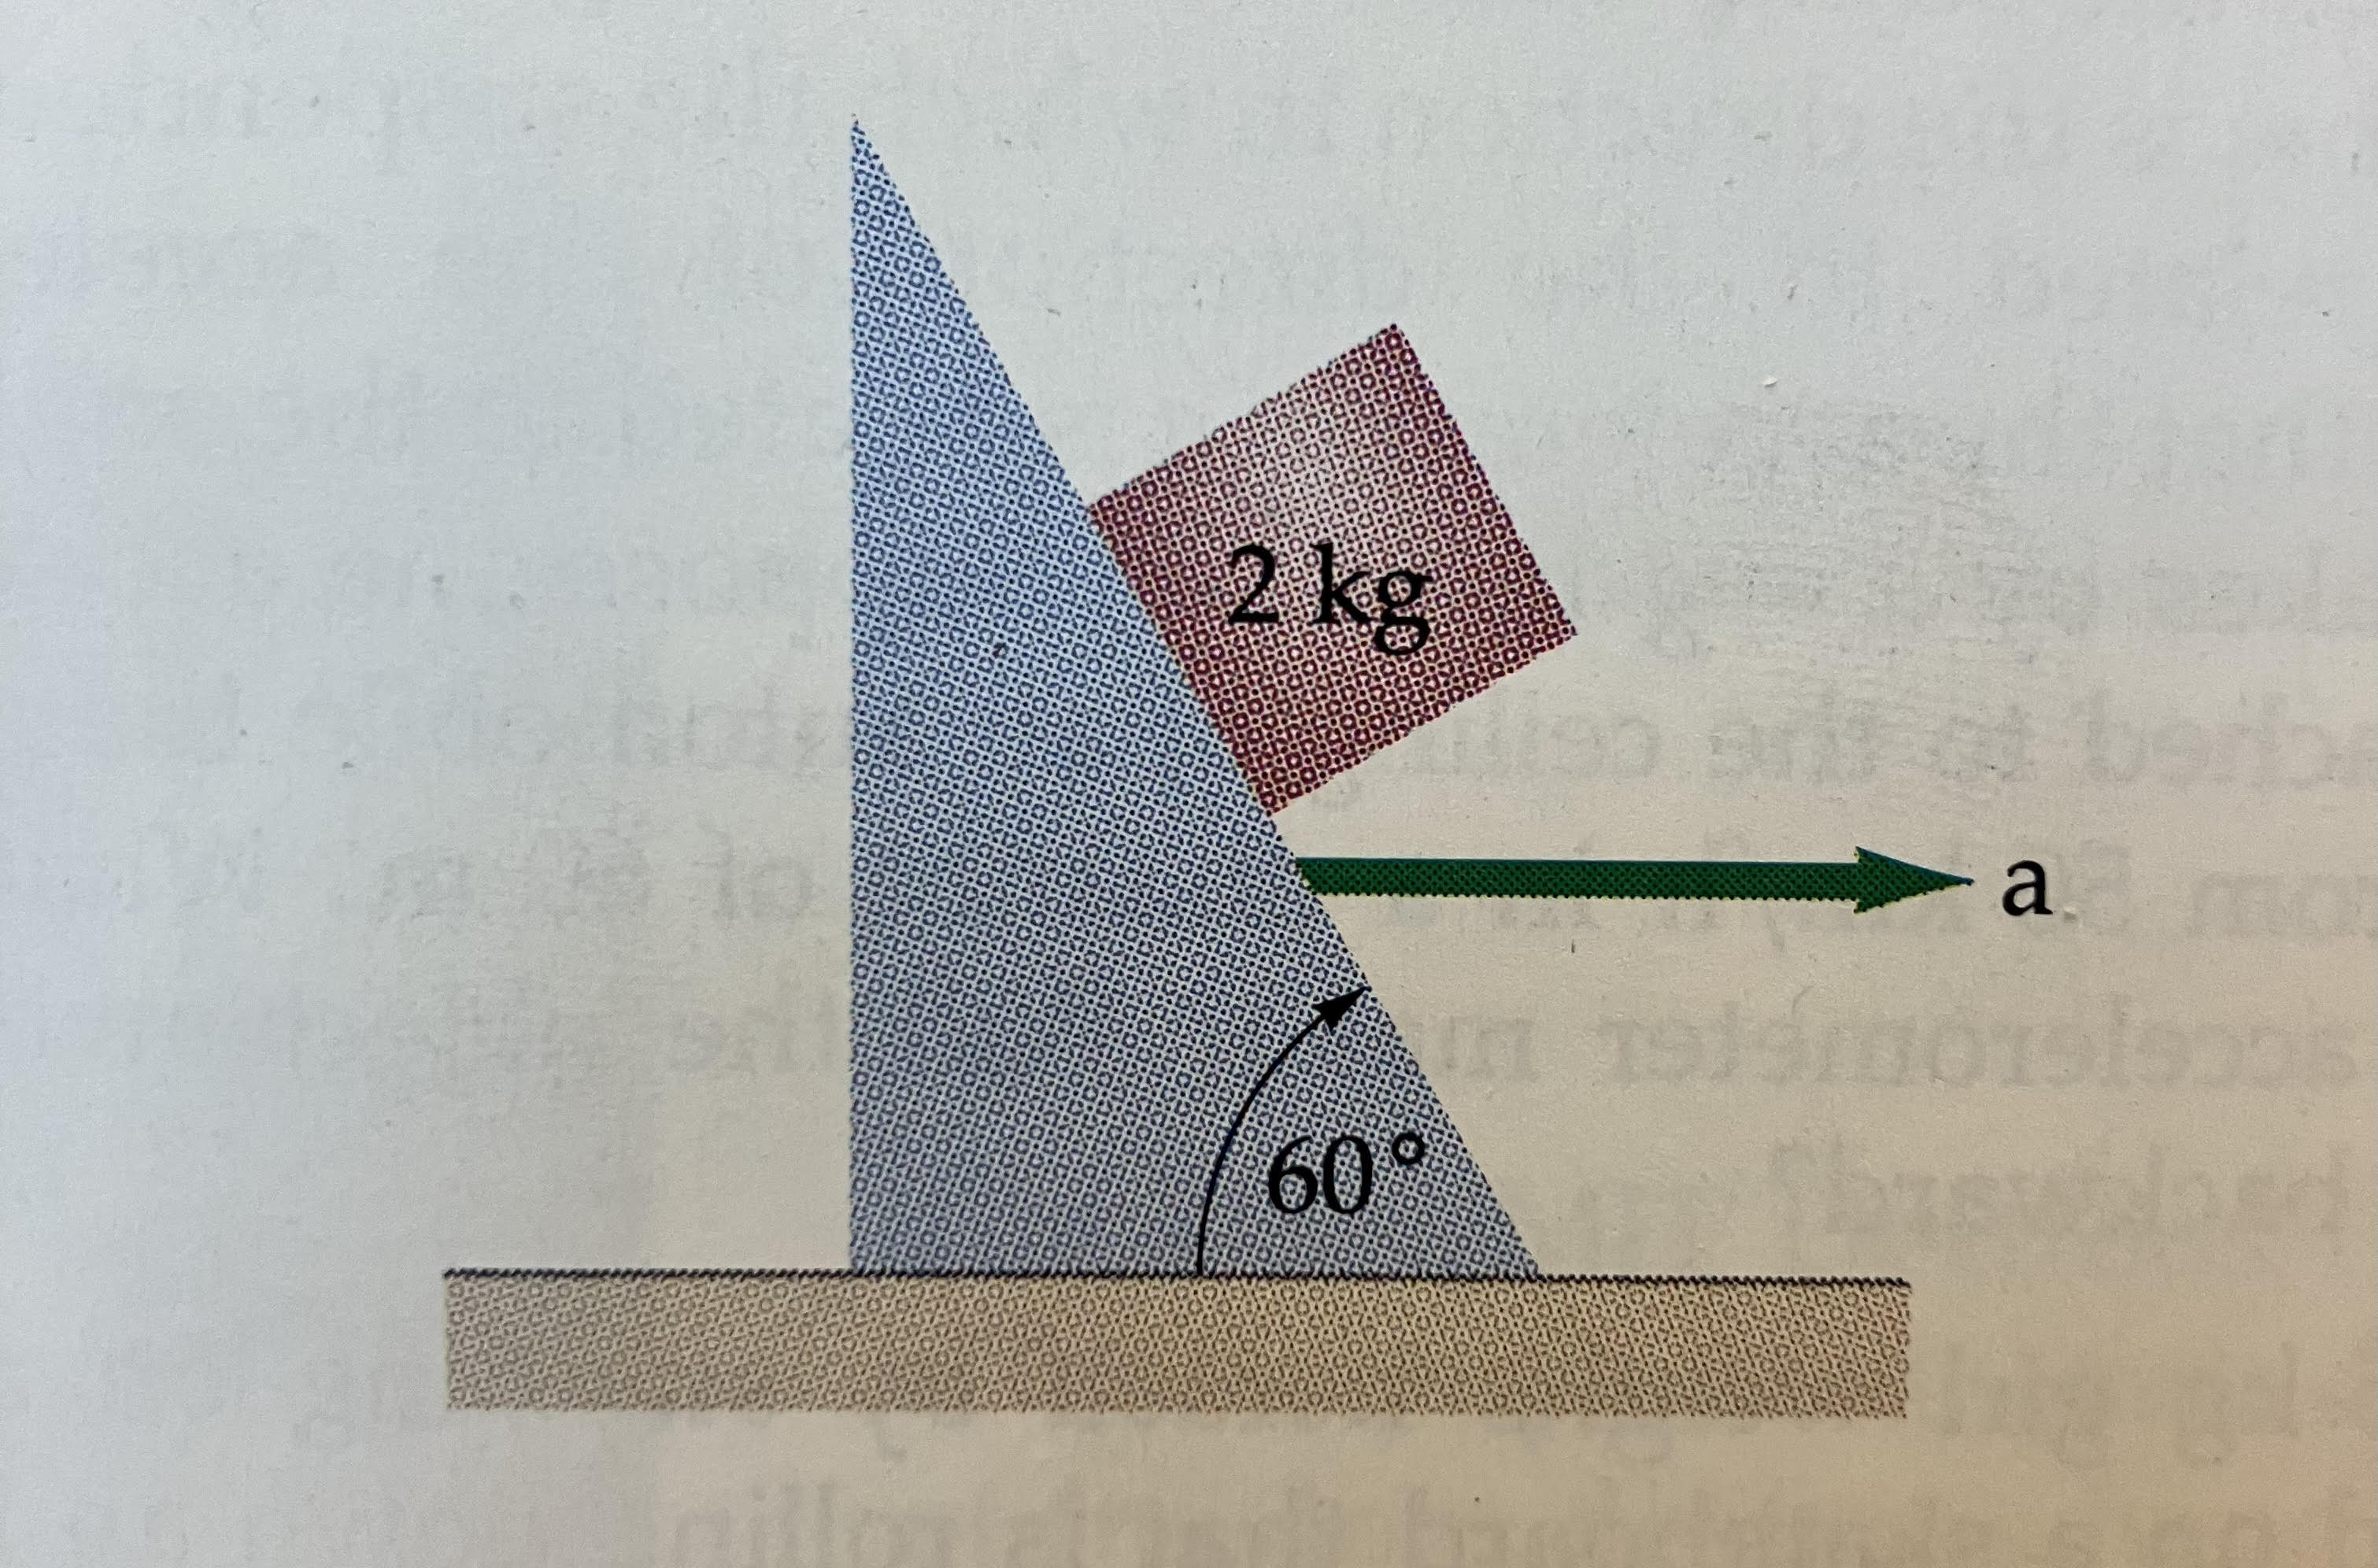
\includegraphics[width=0.5\textwidth]{./exam1_3.jpg}

(a) Determine the acceleration $a$ so that the block remains stationary relative to the wedge. (I recommend orienting the coordinate system so that $x$ is horizontal and $y$ is vertical, in which case there is no acceleration in the $y$-direction.) [4 pts]

\sol{There are two forces acting on the block: gravity, which points downward, and the normal force, which points perpendicular to the block. Summing the forces on the block gives two equations:
\begin{equation}
\sum F_x = N\sin\theta = ma
\end{equation}
\begin{equation}
\sum F_y = N\cos\theta-F_g = 0 \Rightarrow N\cos\theta = mg
\end{equation}
Note that there is no acceleration in the $y$-direction if the block moves horizontally with the wedge. Dividing the first equation by the second equation gives
\begin{equation}
\tan\theta = \frac{a}{g} \Rightarrow \boxed{a=g\tan\theta = 17\mbox{ m/s}^2}
\end{equation}

(b) If the acceleration is larger than 17~m/s$^2$, the block will slide upward, and if the acceleration is less than 17~m/s$^2$ it will slide downward.

}

\clearpage
4. A sprinter running at 9~m/s is 40~m behind a motorcycle that is at rest. At that instant, the motorcycle starts to accelerate at 0.9~m/s$^2$ in the same direction that the sprinter is running. How long does it take for the sprinter to catch the motorcycle, and for how long is the sprinter ahead of the motorcycle? [6 pts]

\sol{The sprinter is running at a constant speed. Their displacement is simply
\begin{equation}
\Delta x_s = v_s\Delta{t}
\end{equation}
The motorcycle is accelerating at a constant rate and has an initial velocity of 0. This means that the displacement of the motorcycle is
\begin{equation}
\Delta x_m = \frac{1}{2}a\Delta t^2
\end{equation}
However, the motorcycle starts some distance, $L$, ahead of the sprinter. Therefore, we need to figure out when does $\Delta x_s = L+\Delta x_m$, and so we set
\begin{equation}
v_s\Delta t = L + \frac{1}{2}a\Delta t^2
\end{equation}
or equivalently,
\begin{equation}
0 = \frac{1}{2}a\Delta t^2 - v_s\Delta t + L
\end{equation}
We can solve for $\Delta t$ using the quadratic equation. The quadratic equation gives us two solutions, $\Delta t = 6.7$~s and $\Delta t=13.3$~s. This means that the sprinter and motorcycle are next to each other at 6.7~s and then again at 13.3~s. In other words, the sprinter catches up to the motorcycle after 6.7~s have passed, and remains ahead for an additional 6.7~s.


}

\clearpage
5. A pitcher throws a fastball at 140~km/h toward home plate, which 18.4~m away. Assume that they throw it horizontally. How far does the ball drop by the time it reaches home plate? [6 pts]

\sol{Use the horizontal motion to figure out the travel time, assuming that $v_x$ is constant and equal to 140~km/h. To convert 140~km/h to m/s, multiple by 1000 and divide by 3600, which gives 38.9~m/s.
\begin{equation}
v_x = \frac{\Delta x}{\Delta t} \Rightarrow \Delta t = \frac{\Delta x}{v_x} = 0.47\mbox{ s}
\end{equation}

Now use this to figure out how far the ball falls. In the $y$-direction,
\begin{equation}
\Delta y = v_{y,i}\Delta t + \frac{1}{2}a_y\Delta t^2
\end{equation}
$v_{y,i}=0$ and $a_y=-g$, so
\begin{equation}
\Delta y = -\frac{1}{2}g\Delta t^2 = \boxed{-1.1\mbox{ m}}
\end{equation}


}



\end{document}


